%======================================================================
\chapter{Hybrid Remote Rendering}
\label{chap:hrr}
%======================================================================

\section{Method}
\label{sec:method}

\subsection{Client-Server Prototype Design}
\label{sec:method:cspd}

Our proposed system aims at providing high-quality rendering on less powerful mobile devices, while minimizing the amount of data transferred via the network. We would also like to enable multi-client cooperation to enhance the user experience in training scenarios.

Our system is inspired by Levoy~\cite{levoy1995}, Lamberti and Sanna~\cite{lamberti2007} and Lu et al.~\cite{lu2011} and uses a hybrid approach incorporating model-based and image-based methods.
On the one hand, the low-fidelity key models are stored on the client-side and the local rendering capacity is leveraged to produce lower quality rendering results.
On the other hand, the high-fidelity rendering results of key models are sent from the server to the client and overlaid upon the locally rendered frames.
Accordingly, the data transferred via the network is minimized due to the small amount of pixels that are sent via the network compared to a CMR solution. 

There are three challenges in realizing multi-client support within the context of the above described system.
First, it is required that the server must not be blocked by any of the clients.
Second, each client has its own view that may be different from all the other clients, this can result in a performance issue as a scene needs to be rendered multiple times in a single animation loop.
Third, because only key models are rendered and sent by the server, occlusion becomes a problem since the environment models that are closer to the viewpoint may not be rendered on the server but just locally.

We address the first problem by mandating that the server interacts with each client independently. More specifically, we enable the server to receive commands from and send to every client seperately, so that if a client becomes unresponsive, the server is not blocked.
The second issue is alleviated by implementing a "render-on-demand" function on the server, which means that the server renders the scene for a client only when the client requires a new frame.
We address the third challenge through a two-pass rendering process. In the first pass, the entire scene is rendered in low fidelity on the server. Then the colour buffer is cleared before the second pass where only the key models are rendered in high fidelity. In this way, the second pass is rendered with the depth information obtained from the first pass.

\begin{figure}[!htbp]
	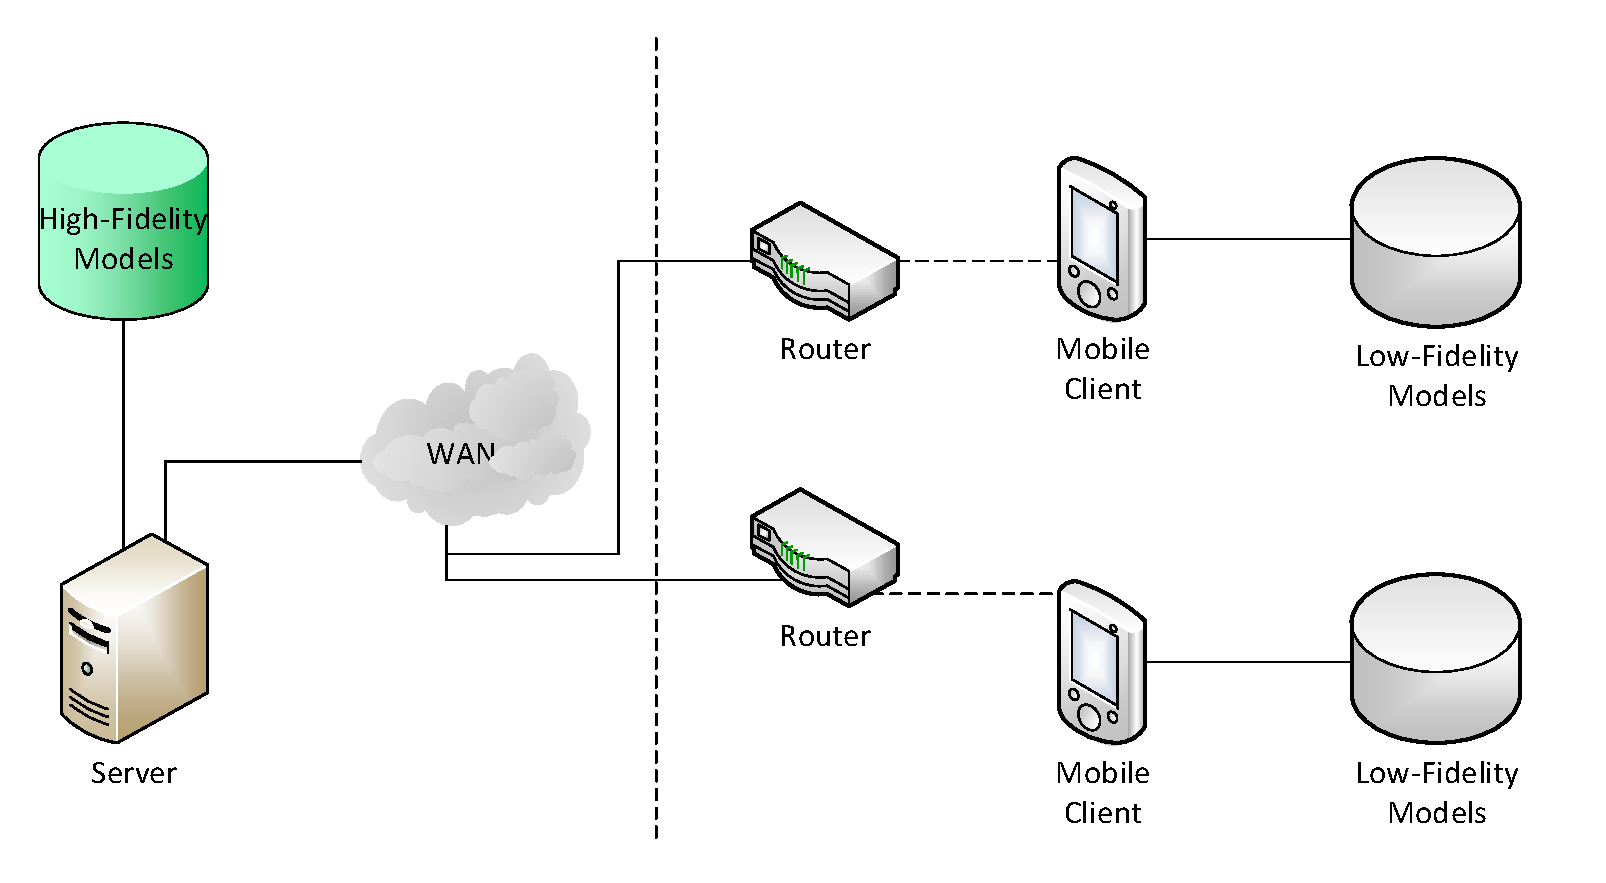
\includegraphics[width=\textwidth]{figures/architecture.pdf}
	\caption{System architecture}
	\label{fig:architecture}
\end{figure}

\begin{figure}[!htbp]
	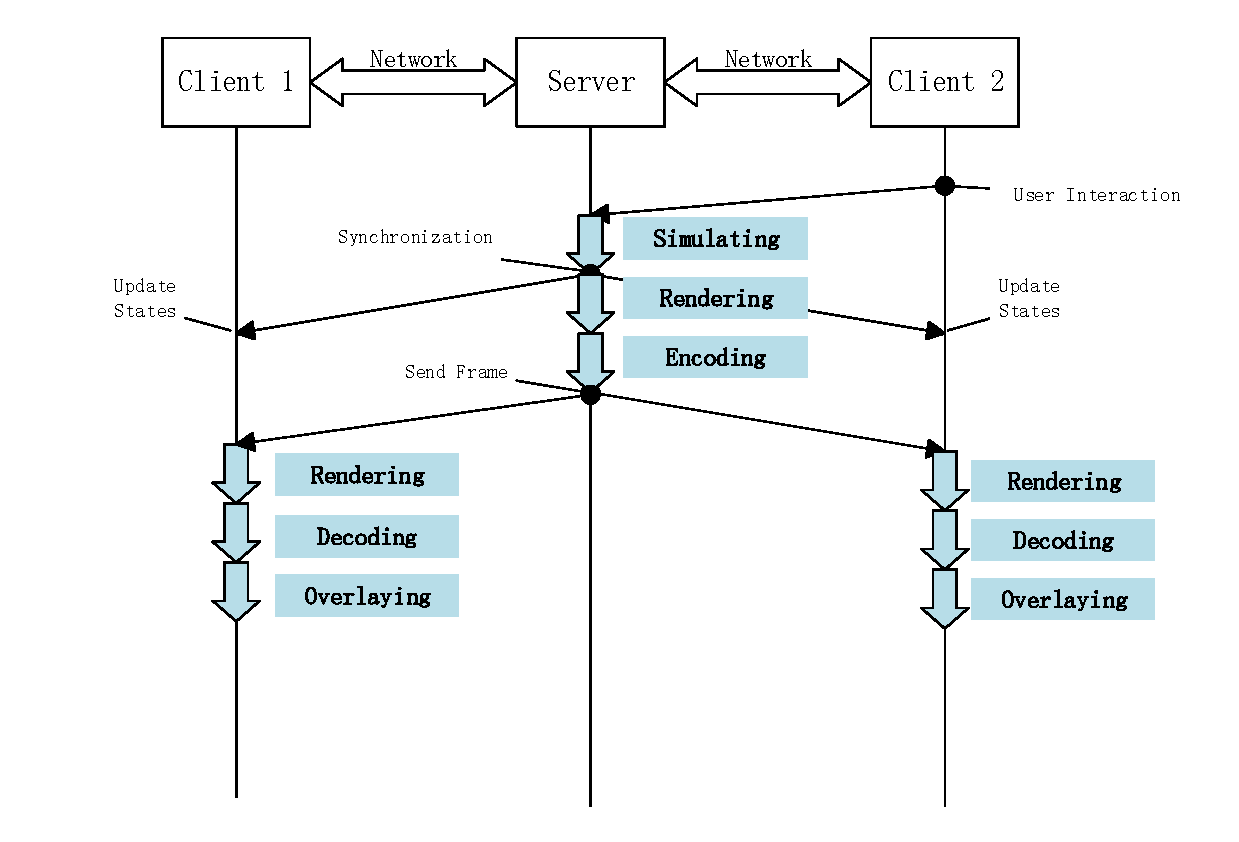
\includegraphics[width=\textwidth]{figures/sequence_workflow.pdf}
	\caption{Workflow of communication between the server and the clients}
	\label{fig:swf}
\end{figure}

As depicted in Fig.~\ref{fig:architecture}, in this system, all clients are connected to the rendering server and send interaction commands to the server.
On the server side, the application status changes according to the commands received from all clients. The application status changes are synchronized with all clients. In this way, the clients are able to cooperate with each other. In other words, when a client changes the status of the application, all clients will see the change after synchronization.
To minimize the amount of transferred data, the client decides which models need to be rendered in high-fidelity and the server only sends the pixels depicting those key models. The other models are still rendered locally.

Fig.~\ref{fig:swf} illustrates the sequence of messages communicated between the server and the clients process. It shows the tasks that are performed by the server and clients to process one frame. If the commands sent from any client influence the simulation states of the server, the latter synchronizes the state changes among all clients to ensure that all of them maintain a consistent state. Moreover, the server renders and encodes the frames for all the clients. Upon receiving the high-fidelity frame, the client decodes and overlays it on the locally rendered frame.

\subsection{Process Behavior}

The proposed system consists of one server and multiple clients.
Fig.~\ref{fig:s-wf} shows the behavior of the server process.
In each loop, the server updates the simulation status of the scene and receives commands from all clients.
Next, the server sends the received commands to all clients to ensure synchronization between them.
On the server side, each client has its own view that is independent from those of the other clients.
The server only renders a new frame upon request from the client.

Fig.~\ref{fig:c-wf} shows the behavior of the client processes. In each loop, the client receives commands from the server and adjusts the simulation status accordingly. Then, it sends its user interaction commands to the server. In each iteration, the client will receive the high-fidelity frame from the server that it has requested in the previous iteration. The client has simplified models stored locally, it renders the scene in every iteration. The high-fidelity frames acquired from the server are overlaid upon the locally rendered frames. Once done, it sends the frame request to the server. In this way, the server does not need to render frames for all clients in every loop, instead it renders a frame when it is needed.

\begin{figure}[!htbp]
	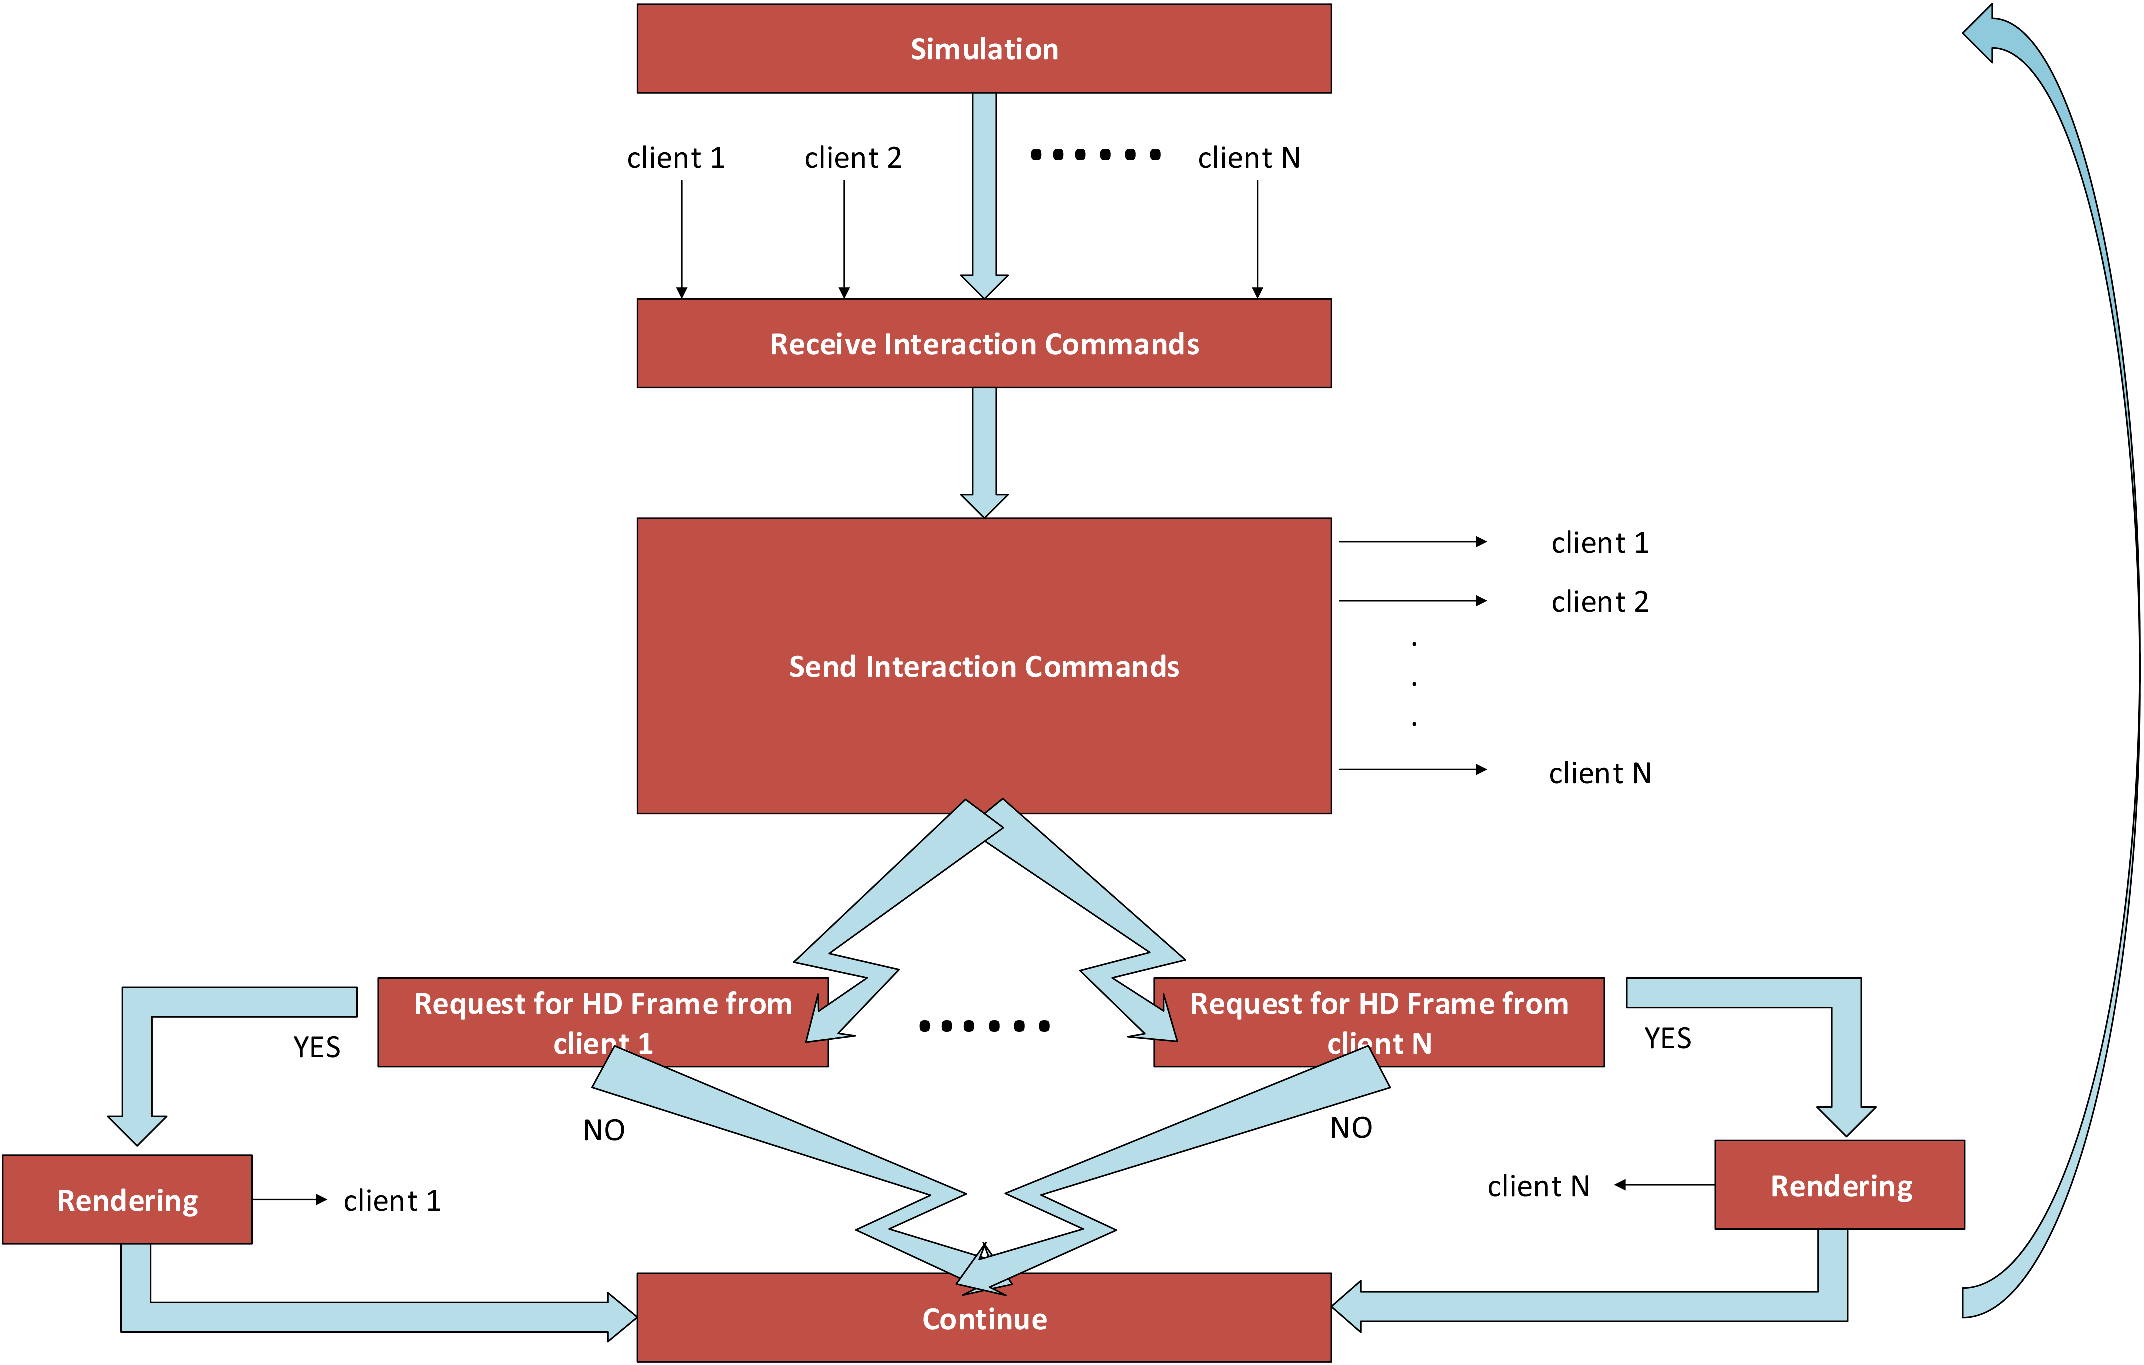
\includegraphics[width=\textwidth]{figures/workflow_server-eps-converted-to.pdf}
	\caption{Server-side Workflow}
	\label{fig:s-wf}
\end{figure}

\begin{figure}[!htbp]
	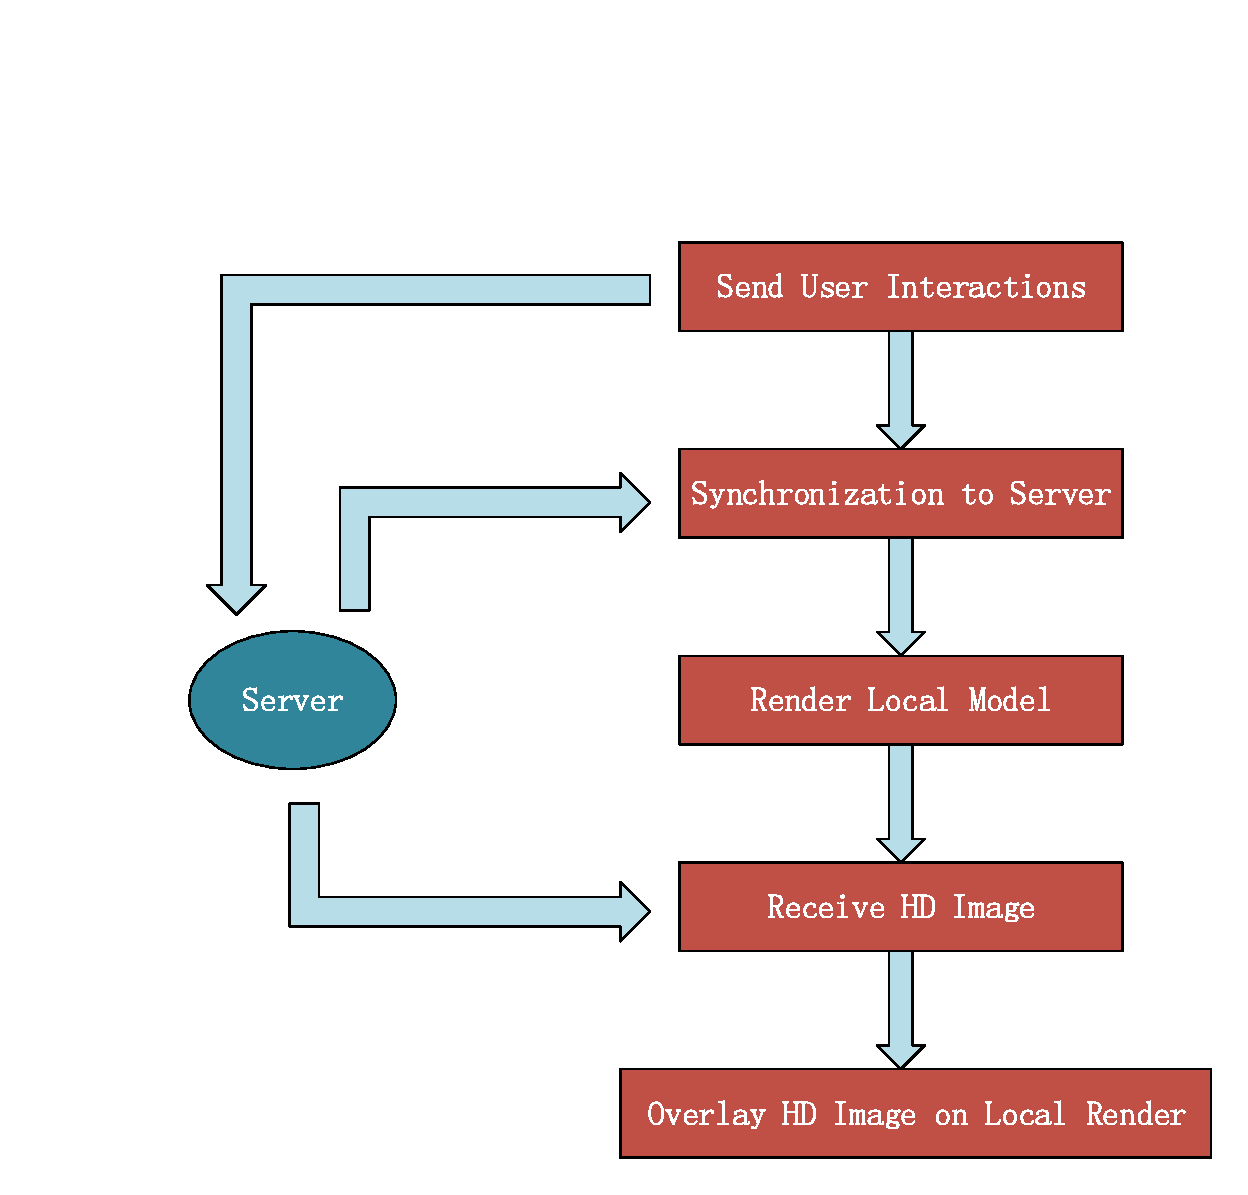
\includegraphics[width=\textwidth]{figures/workflow_client.pdf}
	\caption{Client-side Workflow}
	\label{fig:c-wf}
\end{figure}

\subsection{Two-pass Rendering}

As mentioned in Section~\ref{sec:method:cspd}, we use a two-pass rendering process on the server side.
The frames sent to the client depict only high-fidelity key models.
But this is not enough for valid view of the 3D scene since other scene content may occlude parts of the key models.
We propose a two-pass rendering process to address this issue.

\begin{figure}[!htbp]
	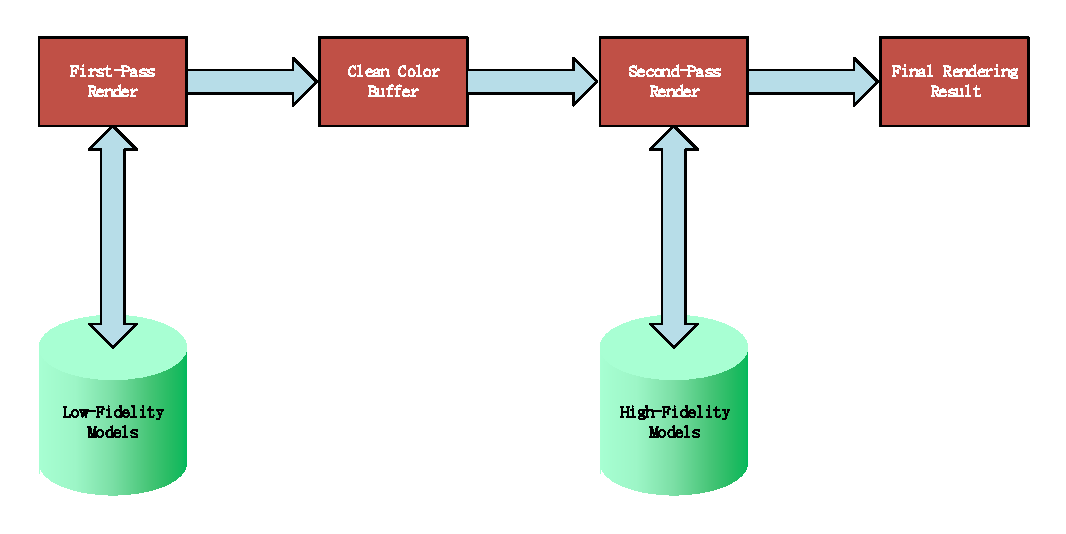
\includegraphics[width=\textwidth]{figures/two-pass-rendering.pdf}
	\caption{Two-pass rendering}
	\label{fig:tp-rendering}
\end{figure}

As shown in Fig.~\ref{fig:tp-rendering}, in the first pass, all models are rendered in low-fidelity except for the key models. Then the color buffer is cleared and only the depth buffer is preserved. In the second pass, only the high-fidelity key models are rendered, while considering the depth information obtained from the first pass rendering, therefore the occlusions are preserved in the final rendered scene.

\section{User Study}
\label{sec:userstudy}

In Section~\ref{sec:method}, we propose a hybrid remote rendering framework that offloads a part of the rendering task to the remote server. More specifically, only key models are rendered remotely to minimize network bandwidth requirement.

To overcome the limitations of mobile devices in rendering high-fidelity models, designers often use one of the two approaches:
\begin{enumerate}
\item
Local-only rendering: Reduce the fidelity of the models and render them locally on mobile devices.
\item
Server-only rendering: Render the scene remotely on a server and transfer to the mobile phone client as a video stream.
\end{enumerate}

However, both approaches risk reducing the user's Quality of Experience (QoE). For the local-only rendering approach, the user is interacting with models that are not rendered at their optimal quality. Fine details in the model might be missing, which reduces the aesthetics of the scene. Also, for some applications, these details might carry important information. For instance, it is important for users in many gaming applications to quickly distinguish between similar objects in a scene. Objects rendered as low-fidelity models might not be immediately discernible. For the server-only approach, QoE might be affected by a long delay between the user's actions and application's response. This would be mostly caused by the network delay between client and server. Furthermore, bandwidth limitations can cause interruptions in the video stream.
The proposed approach strikes a balance between local-only rendering and server-only rendering. It renders only key models remotely at high-fidelity while other models are rendered locally at low-fidelity. 

The previous work have explored how various factors affect the user experience. Hong et al.~\cite{hong2015user-study} conducted a subjective user study to quantify the effect that video bitrate and frame rate have on QoE in cloud gaming.
Slivar et al.~\cite{slivar2015qoe} use Steam In-home streaming platform~\cite{steam-in-home} as a case to study how the frame rate and bitrate influence the QoE.
In the work by Suznjevic et al.~\cite{suznjevic2016}, five factors (i.e. latency, jitter, packet loss, frame rate and frame resolution) are studied in terms of their effects on the QoE of NVIDIA GeForce Now platform~\cite{nvidia-geforce-now}.
We are interested in understanding the consequence of applying this proposed approach on QoE and user performance for a task. The details of this task are provided in Section~\ref{sec:ms}.
Therefore, we conduct a comprehensive user study to assess the impact of a different set of factors than previous work, i.e. network delay, jitter, and the use of low/high-fidelity models.
Hemmati et al.~\cite{hemmati2013bitrate} developed an algorithm that minimizes bitrate through not rendering unimportant models. However, they did not answer the question about how this approach influences user experience. Our method leverages a similar idea that renders key models in high fidelity and environment models in low fidelity. Thus we explore the effect that key model fidelity and environment fidelity have.
Moreover, we are also interested in understanding how our approach affects the user performance on users' object recognition.
In our user study, we do not consider any network-aware adaption strategies of the video stream performed by the remote server.  

In this evaluation, we address the following research questions:
\begin{enumerate}
\item
What is the effect of key model fidelity on the user QoE and performance?
\item
What is the effect of environment model fidelity on the user QoE and performance?
\item
What is the effect of network delay and jitter on the user QoE and performance?
\end{enumerate}

This user study was approved by the Research Ethics Board at the University of Ottawa (File Number: H12-16-05).
The main user study is informed by a pre-trial study discussed next.

\subsection{Pre-Trial Study}
\label{sec:pts}

A major goal of the main study is to analyze the effect of 3D model fidelity on the ability of a user to recognize an object and its impact on the QoE. However, in the proposed framework, there are two types of models, high-fidelity models and low-fidelity models. Those models will be used in the main study (see Section~\ref{sec:ms}). We have prepared 15 high-fidelity models and simplified them to obtain low-fidelity models using QSlim~\cite{garland1997}.

\subsubsection{Objective}

The objective of the pre-trial study is to decide on the number of polygons for the low-fidelity models. If it is too low, the participants will not be able to recognize the object that the model represents. In the pre-trial study, we want to find out at which point the object represented by the model becomes discernible to the majority or all subjects.

\subsubsection{Participants}

We recruited 5 participants, 4 males and 1 female. None of the subjects were visually impaired.

\subsubsection{Independent Variables and Dependent Measures}
\label{sec:ivdm}

The experiment was conducted with one independent variable: number of polygons of the surface mesh in the 3D model.
The independent variable has 50 levels. For the first level, the model is composed of 20 polygons. For each of the 49 subsequent levels, the number of polygons is increased by $10\%$. We measure the number of polygons necessary for a subject to recognize the object for each 3D model.

\subsubsection{Procedure}

The experiment was conducted using a program that shows 15 models at different levels of fidelity.  We create 50 levels of fidelity for each model by starting with a high-fidelity model and decreasing its polygon count by $10\%$ for every level using QSlim~\cite{garland1997}. Our program shows the subjects a model on the screen and asks them to select the object it represents from a side menu by choosing between dog, cat, horse, or unknown. Subjects were instructed to choose the unknown option if they were unsure. We start with a model with very low polygon count (20 polygons). Every time the subject selects an answer, we increase the polygon count to the next level adding more details to the model. The order through which the models are shown to the subjects is randomized to avoid biasing the results. 

\subsubsection{Results}

\begin{table}[!htbp]
\caption{Data collected from the pre-trial study. The number of polygons above which a participant ceases to make mistakes are shown. However, in one case, one of the participants does not recognize the model even at full resolution (marked by a dash). The numbers in bold are those selected as the final number of polygons of the low-fidelity models for the main study.}
\label{tab:pts}
\begin{tabular}{llllll}
\hline\noalign{\smallskip}
& Participant \#1 & Participant \#2 & Participant \#3 & Participant \#4 & Participant \#5 \\
\noalign{\smallskip}\hline\noalign{\smallskip}
Model \#1 & 148 & 22 & 57 & 51 & \textbf{111} \\
Model \#2 & 162 & 57 & \textbf{422} & 22 & 422 \\
Model \#3 & 122 & 383 & 134 & 22 & \textbf{238} \\
Model \#4 & 75 & \textbf{148} & - & 69 & 134 \\
Model \#5 & 162 & 51 & 32 & 22 & \textbf{134} \\
Model \#6 & \textbf{1095} & 179 & 464 & 1940 & 464 \\
Model \#7 & 995 & 1603 & \textbf{1325} & 32 & 422 \\
Model \#8 & 75 & 162 & 148 & 91 & \textbf{148} \\
Model \#9 & 75 & 83 & 216 & 122 & \textbf{196} \\
Model \#10 & 464 & 262 & 748 & 216 & \textbf{562} \\
Model \#11 & 422 & 1204 & \textbf{422} & 288 & 383 \\
Model \#12 & 47 & 101 & \textbf{134} & 22 & 134 \\
Model \#13 & 22 & 47 & 510 & 29 & \textbf{238} \\
Model \#14 & 238 & 22 & 348 & \textbf{317} & 162 \\
Model \#15 & 69 & 83 & \textbf{75} & 75 & 51 \\
\noalign{\smallskip}\hline
\end{tabular}
\end{table}

Table~\ref{tab:pts} contains the data collected from the pre-trial study. The number of polygons above which a participant ceases to make mistakes (i.e. the participant choses the correct answer consistently at all further levels of fidelity). The data are used to decide the number of polygons for the low-fidelity models in the main study. To eliminate the outliers, we select the second highest number among all participants for each model.
% The digits with stars in Table~\ref{tab:pts} demonstrates the final number of polygons of each low-fidelity model.

\subsection{Main Study}
\label{sec:ms}

Our main user study is designed to address the research questions described at the beginning of Section~\ref{sec:userstudy}.
We ask the subjects to interact with a 3D mobile application that prompts the user to respond rapidly to visual stimuli. This is a stand-in for a variety of applications that require the user to react swiftly to changing aspects in a 3D environment. Examples of such applications are games, flight simulators, military training systems, etc... We compare our results to conventional video streaming and local-only rendering approaches.

\subsubsection{Hypothesis}

We devise eight null hypotheses to test in the experiment, see Table~\ref{tab:hypo}. The null hypotheses are defined for each measurement factor. In those null hypotheses, we assume all four factors do not have any effect on the user performance nor the QoE. Rejecting a null hypothesis indicates that the corresponding factor has an effect on that dependent measure.

\begin{table}[!htbp]
\caption{Hypotheses.}
\label{tab:hypo}
\begin{tabular}{ll}
\noalign{\smallskip}\hline\noalign{\smallskip}
H\textsubscript{01} & Different model fidelities do not affect the user performance in recognizing objects \\
H\textsubscript{02} & Different environment fidelities do not affect the user performance in recognizing objects \\
H\textsubscript{03} & Different network delays do not affect the user performance in recognizing objects \\
H\textsubscript{04} & Existence of jitter does not affect the user performance in recognizing objects \\
H\textsubscript{05} & Different model fidelities do not affect the QoE \\
H\textsubscript{06} & Different environment fidelities do not affect the QoE \\
H\textsubscript{07} & Different network delays do not affect the QoE \\
H\textsubscript{08} & Existence of jitter does not affect the QoE \\
\noalign{\smallskip}\hline
\end{tabular}
\end{table}

\subsubsection{Participants}

15 volunteers participated in the main study, 12 males and 3 females. None of the subjects were visually impaired.

\subsubsection{Independent Variables and Dependent Measures}
\label{sec:ms:ivdm}

The experiment was conducted with four independent variables: key model fidelity, environment model fidelity, delay and jitter.
Key model fidelity and environment model fidelity have two levels: high and low, as described in Section~\ref{sec:pts}.
The variable delay is set to introduce network delay. In the variable network delay, we summarize the effects of network transmission, remote rendering and encoding. In this experiment, the variable delay was simulated locally. Similar to the work by Zhu et al.~\cite{zhu1998jitter}, we use a normal distribution for jitter in settings with non-zero delay

\begin{equation}
p(j|\mu,\sigma^{2})=\frac{1}{\sqrt{2\pi\sigma^{2}}}^{-\frac{(j-\mu)^{2}}{2\sigma^{2}}}
\end{equation}
where j is the value of jitter, $\mu=77\mathrm{ms}$ and $\sigma^{2}=1$.

Combining the four variables results in 20 configurations. Table~\ref{tab:pus} details the test application configurations. The order of the 20 configurations is randomized across subjects to avoid biasing the results.

\begin{table}[!htbp]
\caption{Test application configurations.}
\label{tab:pus}
\begin{tabular}{lllll}
\hline\noalign{\smallskip}
Configuration & Key Model Fidelity & Environment Model Fidelity & Delay & Jitter \\
\noalign{\smallskip}\hline\noalign{\smallskip}
1 & low & low & $0\mathrm{ms}$ & not applicable \\
2 & low & high & $0\mathrm{ms}$ & not applicable \\
3 & high & low & $0\mathrm{ms}$ & not applicable \\
4 & high & high & $0\mathrm{ms}$ & not applicable \\
5 & low & low & $80\mathrm{ms}$ & not applied \\
6 & low & high & $80\mathrm{ms}$ & not applied \\
7 & high & low & $80\mathrm{ms}$ & not applied \\
8 & high & high & $80\mathrm{ms}$ & not applied \\
9 & low & low & $80\mathrm{ms}$ & applied \\
10 & low & high & $80\mathrm{ms}$ & applied \\
11 & high & low & $80\mathrm{ms}$ & applied \\
12 & high & high & $80\mathrm{ms}$ & applied \\
13 & low & low & $120\mathrm{ms}$ & not applied \\
14 & low & high & $120\mathrm{ms}$ & not applied \\
15 & high & low & $120\mathrm{ms}$ & not applied \\
16 & high & high & $120\mathrm{ms}$ & not applied \\
17 & low & low & $120\mathrm{ms}$ & applied \\
18 & low & high & $120\mathrm{ms}$ & applied \\
19 & high & low & $120\mathrm{ms}$ & applied \\
20 & high & high & $120\mathrm{ms}$ & applied \\
\noalign{\smallskip}\hline
\end{tabular}
\end{table}

In this experiment, we collect two types of data: QoE and user performance.
The user performance is measured by the number of objects participants successfully recognize.
The QoE is measured using a Mean Opinion Score (MOS) questionnaire. The questionnaire contains one question: "Please score the difficulty to distinguish the objects". A 5 point Likert Scale is used to collect the answers. A score between 1 to 5 is associated with each question, where 1 represents the option "Very Difficult" and 5 represents the option "Very Easy". The mean of all scores is calculated to obtain the MOS. The MOS is collected through a form directly integrated within the test application.

\subsubsection{Procedure}

The test application we use in our experiments depicts a 3D environment representing a virtual room. Guided by an arrow, the user must navigate the environment to reach a destination at which an object will appear and disappear within a short period of time. The user must press on the object before it disappears to bring up a menu prompting her/him to specify the type of that object, as shown in Fig.~\ref{fig:us}.

We run the test application 20 times for each subject. We vary the key model fidelity, environment model fidelity, delay and jitter across these runs. Table~\ref{tab:pus} details the test application configurations for the 20 runs. The order of the 20 configurations is randomized across subjects to avoid biasing the results.
For each configuration, ten 3D objects appear. So the maximum score of user performance for each configuration is 10 and the minimum score is 0.
As mentioned in Section~\ref{sec:ms:ivdm}, we also collect MOS during the experiment. After each run of the test application, the participant was asked to fill the MOS questionnaire.

As shown in Table~\ref{tab:pus}, we prepare four types of scenes: a scene with only low-fidelity key models and low-fidelity environment models, a scene with low-fidelity key models and high-fidelity environment models, a scene with high-fidelity key models and low-fidelity environment models and a scene with high-fidelity key models and high-fidelity environment models. We simulate three different network delays: $0\mathrm{ms}$, $80\mathrm{ms}$ and $120\mathrm{ms}$ and we also consider network jitter.

\begin{figure}[!htbp]
	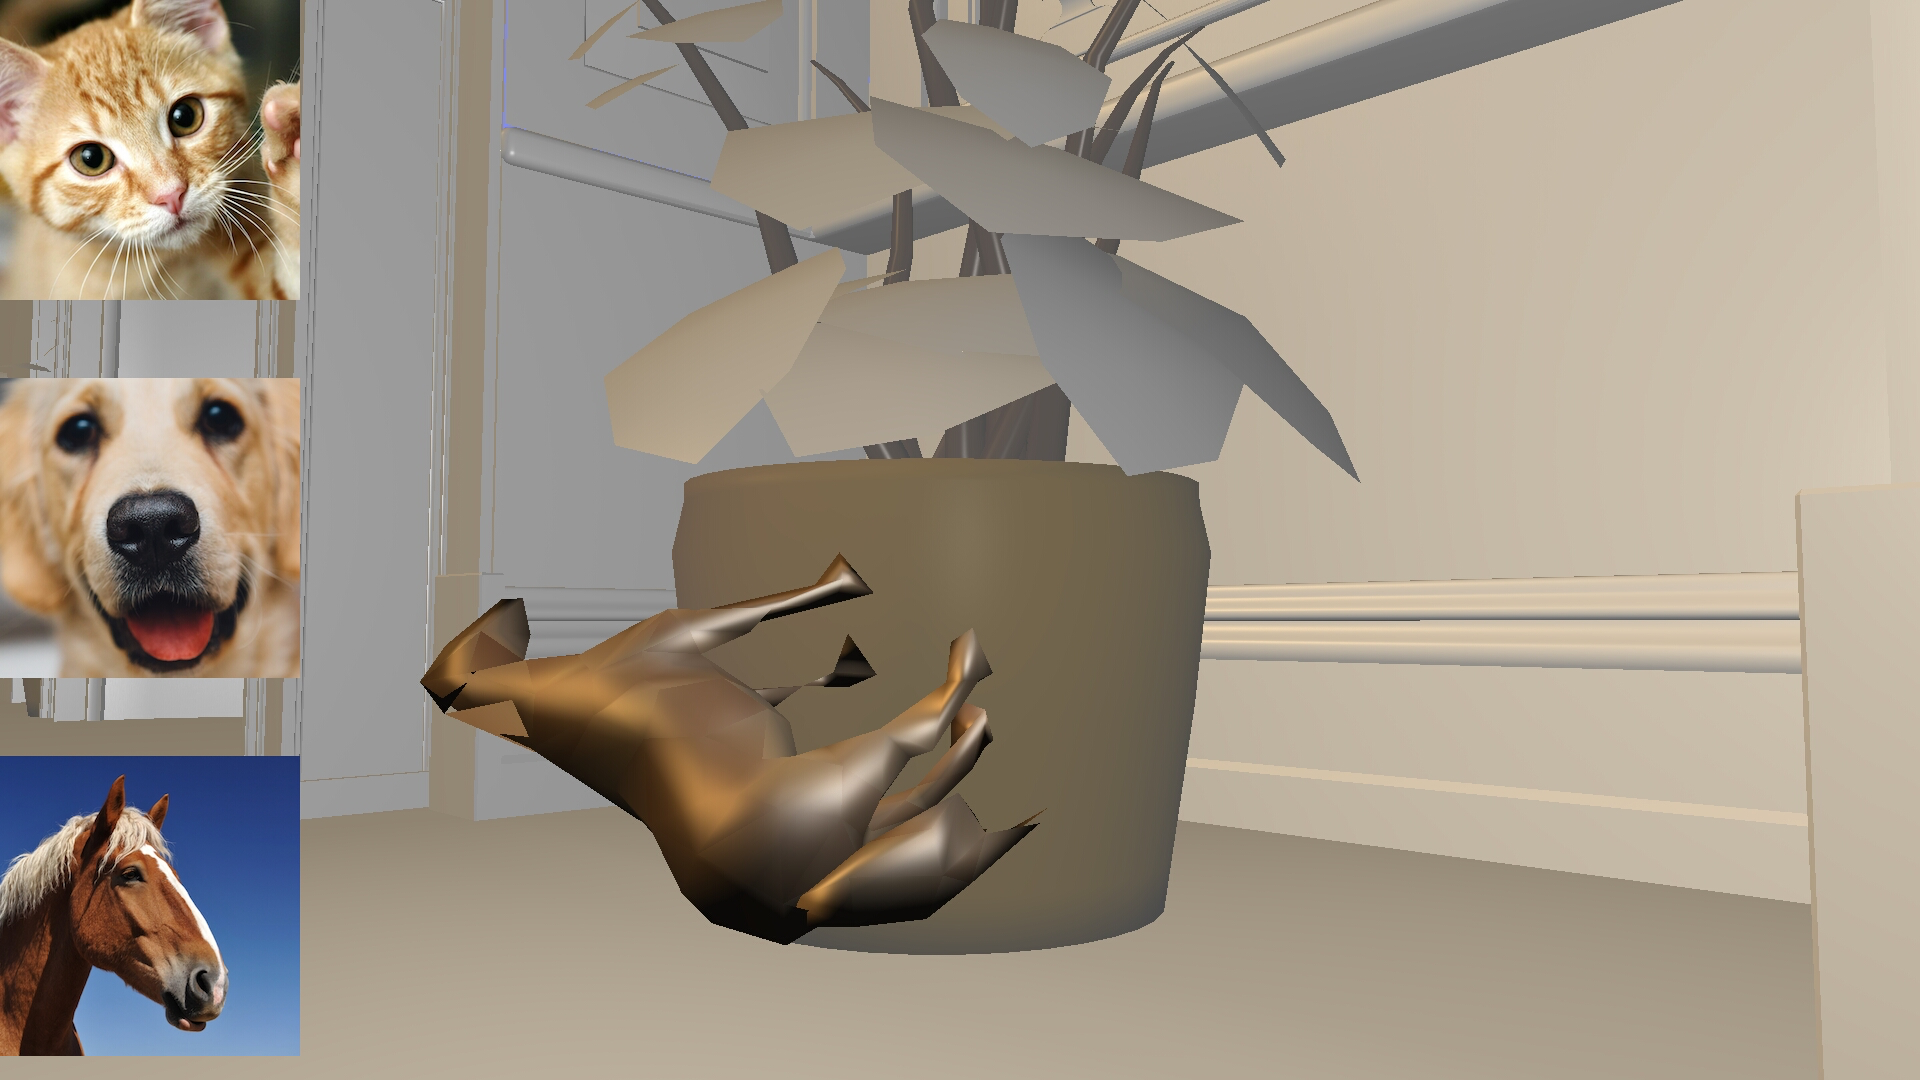
\includegraphics[width=\textwidth]{figures/user_study.png}
	\caption{Screenshot of the application used in the main user study.}
	\label{fig:us}
\end{figure}

\subsubsection{Results}
\label{sec:dao}

To understand how each factor affects MOS and user performance, we use analysis of variance (ANOVA) to interpret our experimental data.

We use a four-way ANOVA test to investigate the effect of all four factors. However the factor combination of delay and jitter is not complete, since jitter is not applicable when delay is $0\mathrm{ms}$. So we exclude the delay level $0\mathrm{ms}$ for the four-way ANOVA test.
As shown in Table~\ref{tab:fal}, the four-way ANOVA considers the four factors and their levels, except for $0\mathrm{ms}$ of delay.

We also analyze the effect of the delay factor and its interaction with key model fidelity and environment model fidelity. For this analysis, we resort to a three-way ANOVA for the combination of delay, key model fidelity and environment model fidelity. Table~\ref{tab:fal} shows the factors of the three way ANOVA.

\begin{table}[!htbp]
\caption{Factors and levels of the ANOVA tests.}
\label{tab:fal}
\begin{tabular}{llllllllll}
\hline\noalign{\smallskip}
& \multicolumn{2}{c}{\makecell{Key Model\\Fidelity}} & \multicolumn{2}{c}{\makecell{Environment\\Model\\Fidelity}} & \multicolumn{3}{c}{Delay} & \multicolumn{2}{c}{Jitter} \\
\noalign{\smallskip}\hline\noalign{\smallskip}
& Low & High & Low & High & $0\mathrm{ms}$ & $80\mathrm{ms}$ & $120\mathrm{ms}$ & applied & not applied \\
\noalign{\smallskip}\hline\noalign{\smallskip}
Four-way ANOVA & \cmark & \cmark & \cmark & \cmark & \xmark & \cmark & \cmark & \cmark & \cmark \\
Three-way ANOVA & \cmark & \cmark & \cmark & \cmark & \cmark & \cmark & \cmark & \xmark & \xmark \\
\noalign{\smallskip}\hline
\end{tabular}
\end{table}

Table.~\ref{tab:mou} shows the grand mean of the user performance measure for all factors. User performance refers to the number of objects the user successfully recognized, hence higher scores represent better performance. Since we employ two tests of significance (four-way and a three-way ANOVA) we calculate two grand means of user performance for each factor level. Four-way ANOVA does not consider the results of configurations 1 to 4 of Table~\ref{tab:pus} (since it does not consider 0ms delay as previously explained).

Table.~\ref{tab:mou} shows that user performance varies with different levels of each factor. However, not all factors have a significant effect on user performance.
We can see that for both, four-way and three-way ANOVA, with high-fidelity key models, participants are able to recognize more objects.
The grand means for the other three factors do not show enough difference between levels of a factor. The differences are not large enough and do not even agree in the four-way ANOVA and three-way ANOVA tests for the factor delay.

Table.~\ref{tab:mom} shows the grand means with respect to MOS. As in Table~\ref{tab:mou}, we show the grand means calculated for the four-way ANOVA and three-way ANOVA tests. The means are measured through a 5 point Likert Scale, where larger values indicate better QoE.

From Table.~\ref{tab:mom}, we can see that reducing network delay clearly improves the QoE, as lower delay levels result in larger MOS scores.
Note that delay is not the only factor that improves the QoE.
With both four-way ANOVA and three-way ANOVA analysis, the participants score their QoE higher with high-fidelity key models over low-fidelity key models (i.e. 2.5 over 2.3 in four-way ANOVA and 2.8 over 2.6 in three-way ANOVA).
However, compared to the differences between levels of network delay, the differences between low key model fidelity and high key model fidelity are relatively small.

\begin{table}[!htbp]
\caption{Grand means of user performance for each factor.}
\label{tab:mou}
\begin{tabular}{llllllllll}
\hline\noalign{\smallskip}
& \multicolumn{2}{c}{\makecell{Key Model\\Fidelity}} & \multicolumn{2}{c}{\makecell{Environment\\Model\\Fidelity}} & \multicolumn{3}{c}{Delay} & \multicolumn{2}{c}{Jitter} \\
\noalign{\smallskip}\hline\noalign{\smallskip}
& low & high & low & high & $0\mathrm{ms}$ & $80\mathrm{ms}$ & $120\mathrm{ms}$ & applied & not applied \\
\noalign{\smallskip}\hline\noalign{\smallskip}
Four-way ANOVA & 5.4 & 6.5 & 6.1 & 5.8 & - & 6.0 & 5.9 & 6.2 & 5.8 \\
Three-way ANOVA & 5.7 & 6.5 & 6.2 & 6.0 & 6.0 & 6.1 & 6.2 & - & - \\
\noalign{\smallskip}\hline
\end{tabular}
\end{table}

\begin{table}[!htbp]
\caption{Grand means of the MOS for each factor.}
\label{tab:mom}
\begin{tabular}{llllllllll}
\hline\noalign{\smallskip}
& \multicolumn{2}{c}{\makecell{Key Model\\Fidelity}} & \multicolumn{2}{c}{\makecell{Environment\\Model\\Fidelity}} & \multicolumn{3}{c}{Delay} & \multicolumn{2}{c}{Jitter} \\
\noalign{\smallskip}\hline\noalign{\smallskip}
& low & high & low & high & $0\mathrm{ms}$ & $80\mathrm{ms}$ & $120\mathrm{ms}$ & applied & not applied \\
\noalign{\smallskip}\hline\noalign{\smallskip}
Four-way ANOVA & 2.3 & 2.5 & 2.3 & 2.4 & - & 2.5 & 2.2 & 2.5 & 2.3 \\
Three-way ANOVA & 2.6 & 2.8 & 2.8 & 2.7 & 3.1 & 2.6 & 2.4 & - & - \\
\noalign{\smallskip}\hline
\end{tabular}
\end{table}

We analyze the variance for both metrics, i.e. user performance and MOS.
To determine whether any of the differences between the means are  statistically significant, we compare the $p$-values to a significance level to accept or reject the null hypothesis. We choose a significance level of 0.05.

Table~\ref{tab:fau} and Table~\ref{tab:tau} demonstrate the results of ANOVA in terms of user performance, where Table~\ref{tab:fau} shows the results of the four way ANOVA while Table~\ref{tab:tau} shows the results of the three way ANOVA.

Only the key model fidelity factor exhibits a $p$-value less than 0.05 for both ANOVA tests for the user performance measure.
To explore the interaction between a factor pair or among multiple factors, we also calculate the $p$-values for those interactions.
These kind of calculations are performed for every combination of factors, including combination of two factors, combination of three factors, and combination of four factors if plausible.
From Table.~\ref{tab:fau} and Table.~\ref{tab:tau}, we can see that there is no combination whose $p$-value is larger than 0.05.
This indicates that these factors are independent from each other in terms of user performance.

\begin{table}[!htbp]
\caption{Four-way ANOVA of user performance.}
\label{tab:fau}
\begin{tabular}{lll}
\hline\noalign{\smallskip}
Source & F-statistics & $p$-value \\
\noalign{\smallskip}\hline\noalign{\smallskip}
Model Fidelity & 14.9 & 0.0001 \\
Environment Model Fidelity & 1.28 & 0.2589 \\
Delay & 0.14 & 0.7063 \\
Jitter & 1.71 & 0.1929 \\
Model Fidelity $\times$ Environment Model Fidelity & 0 & 0.9769 \\
Model Fidelity $\times$ Delay & 0.14 & 0.7063 \\
Model Fidelity $\times$ Jitter & 0.24 & 0.6223 \\
Environment Model Fidelity $\times$ Delay & 0.24 & 0.6223 \\
Environment Model Fidelity $\times$ Jitter & 1.03 & 0.3109 \\
Delay $\times$ Jitter & 0.53 & 0.4689 \\
Model Fidelity $\times$ Environment Model Fidelity $\times$ Delay & 2.93 & 0.0882 \\
Model Fidelity $\times$ Environment Model Fidelity $\times$ Jitter & 0.37 & 0.5429 \\
Model Fidelity $\times$ Delay $\times$ Jitter & 0.04 & 0.8392 \\
Environment Model Fidelity $\times$ Delay $\times$ Jitter & 3.13 & 0.0781 \\
Model Fidelity $\times$ Environment Model Fidelity $\times$ Delay $\times$ Jitter & 1.28 & 0.2589 \\
\noalign{\smallskip}\hline
\end{tabular}
\end{table}

\begin{table}[!htbp]
\caption{Three-way ANOVA of user performance.}
\label{tab:tau}
\begin{tabular}{lll}
\hline\noalign{\smallskip}
Source & F-statistics & $p$-value \\
\noalign{\smallskip}\hline\noalign{\smallskip}
Model Fidelity & 6.33 & 0.0128 \\
Environment Model Fidelity & 0.12 & 0.7342 \\
Delay & 0.12 & 0.8826 \\
Model Fidelity $\times$ Environment Model Fidelity & 004 & 0.8385 \\
Model Fidelity $\times$ Delay & 0.28 & 0.7544 \\
Environment Model Fidelity $\times$ Delay & 0.48 & 0.6217 \\
Model Fidelity $\times$ Environment Model Fidelity $\times$ Delay & 0.6 & 0.5517 \\
\noalign{\smallskip}\hline
\end{tabular}
\end{table}

Table.~\ref{tab:fam} shows the results of four-way ANOVA for the MOS measure, and Table.~\ref{tab:tam} shows the results of three-way ANOVA test.
As opposed to the tests of significance for the performance measure, for the MOS, the model fidelity is not significant. Instead, the delay factor is statistically significant (with a $p$-value of 0.0281 for the four-way ANOVA test and 0.0018 for the three-way ANOVA test).

Further more, we analyze the interaction for factor combinations (just like what we did for the performance measure).
The results demonstrate that there is no interaction between the four factors.

\begin{table}[!htbp]
\caption{Four-way ANOVA of MOS.}
\label{tab:fam}
\begin{tabular}{llllll}
\hline\noalign{\smallskip}
Source & F-statistics & $p$-value \\
\noalign{\smallskip}\hline\noalign{\smallskip}
Model Fidelity & 2.95 & 0.0871 \\
Environment Model Fidelity & 0.96 & 0.3271 \\
Delay & 4.88 & 0.0281 \\
Jitter & 2.95 & 0.0871 \\
Model Fidelity $\times$ Environment Model Fidelity & 0.38 & 0.54 \\
Model Fidelity $\times$ Delay & 0.02 & 0.9024 \\
Model Fidelity $\times$ Jitter & 0.38 & 0.54 \\
Environment Model Fidelity $\times$ Delay & 1.22 & 0.2704 \\
Environment Model Fidelity $\times$ Jitter & 1.82 & 0.1783 \\
Delay $\times$ Jitter & 0.74 & 0.3911 \\
Model Fidelity $\times$ Environment Model Fidelity $\times$ Delay & 0.24 & 0.6239 \\
Model Fidelity $\times$ Environment Model Fidelity $\times$ Jitter & 0.54 & 0.4622 \\
Model Fidelity $\times$ Delay $\times$ Jitter & 0.54 & 0.4622 \\
Environment Model Fidelity $\times$ Delay $\times$ Jitter & 2.95 & 0.0871 \\
Model Fidelity $\times$ Environment Model Fidelity $\times$ Delay $\times$ Jitter & 3.39 & 0.0669 \\
\noalign{\smallskip}\hline
\end{tabular}
\end{table}

\begin{table}[!htbp]
\caption{Three-way ANOVA of MOS.}
\label{tab:tam}
\begin{tabular}{llllll}
\hline\noalign{\smallskip}
Source & F-statistics & $p$-value \\
\noalign{\smallskip}\hline\noalign{\smallskip}
Model Fidelity & 1.2 & 0.2743 \\
Environment Model Fidelity & 0.34 & 0.5623 \\
Delay & 6.55 & 0.0018 \\
Model Fidelity $\times$ Environment Model Fidelity & 0.04 & 0.8468 \\
Model Fidelity $\times$ Delay & 0.7 & 0.4964 \\
Environment Model Fidelity $\times$ Delay & 0.16 & 0.8503 \\
Model Fidelity $\times$ Environment Model Fidelity $\times$ Delay & 0.46 & 0.6309 \\
\noalign{\smallskip}\hline
\end{tabular}
\end{table}

Given the results obtained with the tests of significance, we conclude that the key model fidelity factor affects user performance significantly, while the delay factor affects the MOS significantly. We could not show any influence of other factors beyond what may occur by chance. Given these results, we render our verdict in regards to the hypotheses declared in Table~\ref{tab:hypo} by either accepting or rejecting each null hypothesis.
H\textsubscript{01} and H\textsubscript{07} are rejected since the key model fidelity and delay factors have significant effect on user performance and QoE respectively.

\begin{table}[!htbp]
\caption{Hypotheses. The third column shows if a hypothesis is accepted or rejected according to }
\label{tab:results}
\begin{tabular}{lll}
\hline\noalign{\smallskip}
H\textsubscript{01} & Different model fidelities do not affect the user performance of recognizing objects & reject \\
H\textsubscript{02} & Different environment fidelities do not affect the user performance of recognizing objects & accept \\
H\textsubscript{03} & Different network delays do not affect the user performance of recognizing objects & accept \\
H\textsubscript{04} & Existence of jitter does not affect the user performance of recognizing objects & accept \\
H\textsubscript{05} & Different model fidelities do not affect the QoE & accept \\
H\textsubscript{06} & Different environment fidelities do not affect the QoE & accept \\
H\textsubscript{07} & Different network delays do not affect the QoE & reject \\
H\textsubscript{08} & Existence of jitter does not affect the QoE & accept \\
\noalign{\smallskip}\hline
\end{tabular}
\end{table}

Now we can answer the three questions asked at the beginning of this section.
\begin{enumerate}
\item
The key model fidelity factor has a significant effect on the user performance. Finer key model fidelity helps the user to achieve better performance. But we could not show a significant effect on the QoE. 
\item
We could not show a significant effect of the environment fidelity factor on the user performance nor the QoE.
\item
The delay factor has a significant effect on the QoE in our study. Longer delay results in worse QoE but it does not have a significant effect on the user performance.
\item
The jitter factor has no significant effect on the user performance nor the QoE.
\end{enumerate}

In conclusion, the user study supports the idea of only rendering and sending key models in remote rendering applications.
First, not rendering the environment models in high fidelity has no significant effect on users' object recognition. In gaming, training, medical visualization and other areas where remote rendering has been used, low-fidelity environments do not prevent users from completing the task.
Second, not rendering and sending the environment to clients saves rendering time and network usage, thus our approach is able to reduce the delay that has a significant effect on the QoE.

\section{Conclusions}

We propose a hybrid remote rendering framework for mobile applications.
It uses a client-server model, where the server is responsible for rendering high-fidelity models, encoding and sending the rendered frames to the client. However, in our approach only key models are rendered on the server and sent to the client. The client uses low-fidelity models to render frames locally and overlays the frames received from the server onto its local rendering frames.
In this way, the client is able to display rendering effects that are not available with mobile graphic devices, with lower bandwidth requirements than in streaming-only solutions.
Moreover, since low-fidelity models are stored and rendered on the client side, our framework is able to adapt to different network conditions, and an application is able to continue to run, even if the network becomes completely unavailable.

We conducted a user study on the factors involved in the proposed framework affecting user experience and performance: key model fidelity, environment model fidelity, delay and jitter. We developed an experimental application in which user are asked to recognize objects in different configurations pertaining to the identified factors. Our user study shows that model fidelity affects a user's ability to recognize objects and that network delay plays an important role in the quality of a user's experience. When streaming over non-dedicated networks, the conditions often do not satisfy the requirements of remote rendering applications. Therefore, trading off between rendering quality and network delay is essential but existing remote rendering applications cannot address this issue in a satisfactory way. The most important contribution of the proposed framework is enabling such a trade-off.
